%==========================
% Chapter 11: Designing Information-Sound Systems
%==========================

\chapter{Designing Information-Sound Systems}

\begin{keyinsight}
Building reliable AI systems is not about chasing the latest architecture or scaling to ever-larger models. It is about organizing how information flows through your system: acquiring what you need and only that, constraining what you produce to prevent drift, keeping feedback loops stable, and allocating resources efficiently. These principles endure across model families and problem domains because they are grounded in the fundamental limits of information itself.
\end{keyinsight}

\vspace{1.5em}

In the previous chapters, we have built a deep understanding of how models learn, compress, and generalize. We have explored the information-theoretic foundations of loss functions, the Bayesian perspective on uncertainty, the geometric structure of probability distributions, and the mathematical guarantees that govern generalization. But understanding these foundations is not the same as building systems that work reliably in production.

This chapter is about the engineering discipline that transforms theoretical understanding into working systems. We will see how the information-theoretic principles from Chapter 1, the Bayesian reasoning from Chapter 2, and the compression-generalization connection from Chapter 9 translate into concrete design patterns for real systems.

The central challenge is this: you have a model that has learned to compress patterns in training data. You need to deploy this model in an environment where inputs may differ from training, where outputs have consequences, and where resources like compute and latency matter. How do you design the scaffolding around the model to ensure it behaves reliably?

The answer is not a single architecture or framework. Different applications require different solutions. But there are recurring patterns that emerge from information-theoretic principles. These patterns are about managing information flow: acquiring evidence when you lack it, constraining outputs to prevent format drift, monitoring for distribution shift, and budgeting resources efficiently.

We will explore five key patterns in this chapter. First, we examine how to acquire information through retrieval when the model's internal knowledge is insufficient. Second, we discuss how to constrain what the model produces through structured outputs and validation. Third, we explore how to keep the system stable by monitoring for drift and designing graceful fallbacks. Fourth, we analyze efficiency: how to allocate limited resources like tokens, latency, and compute. Finally, we synthesize these patterns into a minimal architecture that captures what endures across different deployment scenarios.

Throughout, we will stay grounded in information theory. Retrieval is about adding evidence to reduce entropy. Constraints are about restricting the output space to high-probability regions. Monitoring is about detecting when distributions shift. Efficiency is about allocating information capacity where it matters most. This perspective helps us see past surface-level implementation details to the underlying principles that govern reliable systems.

\vspace{2em}

%==========================
\section{Acquire What You Need (and Only That)}
%==========================

Let's start with a fundamental question: when should you retrieve additional information, and when should you trust what the model already knows? This is not just an engineering question about when to query a database or vector store. It is a question about Bayesian evidence and how much uncertainty reduction you get from external information.

\vspace{1em}

\subsection{Retrieval as Evidence Acquisition}

Think about retrieval through the lens we developed in Chapter 2. Your model has a prior distribution over possible answers based on its training data. When you retrieve relevant documents or facts, you are acquiring evidence that updates this prior into a posterior. The question is: how much does the posterior differ from the prior, and is that difference worth the cost?

From an information-theoretic perspective, retrieval is valuable when it reduces entropy significantly. Suppose your model's prior over possible answers has high entropy because many answers seem plausible. A well-chosen retrieval can concentrate probability mass on the correct answer, reducing entropy dramatically. Conversely, if your model's prior is already highly concentrated on the right answer, retrieval adds little information and may not be worth the latency and compute cost.

Let me make this concrete. Suppose you ask a language model "What is the capital of France?" The model's prior, based on training, assigns probability 0.999 to "Paris" and spreads the remaining 0.001 over other cities. The entropy is very low: $H = -0.999 \log(0.999) - 0.001 \log(0.001) \approx 0.011$ nats. Retrieving a document that says "Paris is the capital of France" changes the posterior negligibly. You have spent retrieval cost for almost no information gain.

Now suppose you ask "What is the current population of Paris?" The model's prior might be a broad distribution over plausible values from 2 million to 12 million, based on when the training data was collected and what the model remembers. Retrieving a recent census document that says "Paris had 2.16 million residents as of 2023" sharply concentrates the posterior around 2.16 million. The entropy drops dramatically, and the retrieval was worth it.

The key insight is that retrieval value depends on the gap between prior entropy and posterior entropy. You should retrieve when this gap is large relative to the cost of retrieval.

\begin{figure}[t]
\centering
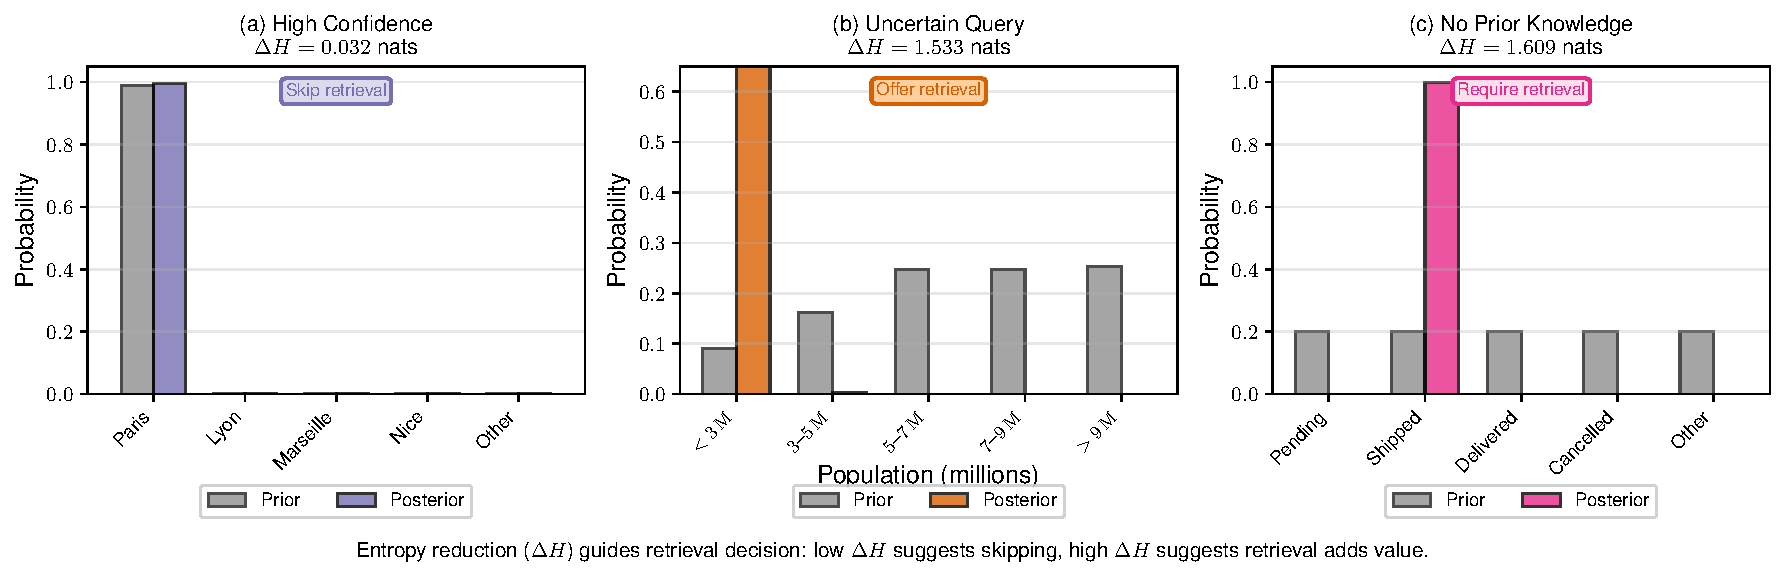
\includegraphics[width=\linewidth]{code/figures/ch11_optimization_geometry/fig_11_1_retrieval_entropy.pdf}
\caption{Entropy reduction guides retrieval: when predictive entropy is low, skip retrieval; when it is high or knowledge is missing, retrieving evidence adds value before generation.}
\label{fig:retrieval_entropy}
\end{figure}

\vspace{1em}

\subsection{When to Fetch Versus When to Trust Priors}

How do you operationalize this principle? You need a way to estimate the model's uncertainty before retrieval. For language models, several signals can serve as proxies:

The model's own output probability distribution over tokens gives you a direct measure of predictive entropy. If the model assigns most probability mass to a single continuation, it is confident. If probability is spread over many continuations, it is uncertain. You can threshold on entropy or use the maximum probability as a confidence score.

The presence of temporal or factual references in the query often signals that retrieval is needed. Questions about "current," "latest," or "recent" information cannot be answered reliably from the model's training distribution. Similarly, questions that reference specific entities, dates, or events benefit from retrieval to ground the answer in verified facts.

The domain and task matter too. For creative generation tasks like storytelling or brainstorming, the model's prior may be all you need because there is no single correct answer. For factual question answering, medical diagnosis, or legal reasoning, external evidence is often critical because correctness matters and the model's training data may be incomplete or outdated.

A practical heuristic is to classify queries into three categories. For high-confidence, closed-domain queries where the answer is well-known and stable over time, trust the model's prior. For low-confidence or open-domain queries where facts are uncertain or rapidly changing, always retrieve. For intermediate cases, use the model's predictive entropy as a trigger: retrieve only when entropy exceeds a threshold.

\vspace{1.5em}

\begin{examplebox}
\textbf{Retrieval Decision Framework}

\vspace{0.5em}

Suppose you are building a customer support chatbot. You receive three queries:

\vspace{0.5em}

\textbf{Query 1: "How do I reset my password?"}

This is a closed-domain, high-frequency question. The model has seen thousands of similar examples in training and knows the standard procedure. Predictive entropy over the first few tokens is low (the model is confident it should start with "To reset your password, go to..."). Decision: do not retrieve. Trust the model's prior.

\vspace{0.5em}

\textbf{Query 2: "What is your return policy for items purchased during the December sale?"}

This references a specific event ("December sale") that may have unique terms. The model's prior over return policies is broad because different sales have different rules. Predictive entropy is moderate to high. Decision: retrieve the specific policy document for the December sale before answering.

\vspace{0.5em}

\textbf{Query 3: "I ordered product XYZ123 last week, where is it?"}

This is about a specific order that the model cannot possibly know about from training. The model's prior over order status is essentially uniform because it has no information. Decision: retrieve the order status from the database. This is mandatory retrieval, not optional.

\vspace{0.5em}

By categorizing queries this way, you allocate retrieval resources efficiently. Most queries fall into the first category and can be answered directly. A smaller fraction requires retrieval, and you focus resources there.
\end{examplebox}

\vspace{1.5em}

\subsection{Chunking, Indexing, and the Curse of Context Length}

Once you decide to retrieve, you face a practical challenge: how do you find the right information and present it to the model efficiently? This is where chunking and indexing come in, and where information theory gives us principled guidance.

The problem is that documents are long, but context windows are finite. Even with large context windows of tens or hundreds of thousands of tokens, you cannot pass entire databases to the model. You need to select relevant chunks and present them in a way that maximizes information density.

Chunking is about dividing documents into units that are small enough to fit in context but large enough to contain coherent information. A chunk that is too small (a single sentence) may lack necessary context. A chunk that is too large (an entire document) wastes context on irrelevant information. The optimal chunk size depends on the typical granularity of queries and answers.

From a compression perspective, good chunks are those that have high mutual information with queries. You want chunks that, when retrieved, sharply reduce the entropy over possible answers. This suggests that chunks should be semantically coherent units: paragraphs, sections, or passages that discuss a single topic. Breaking mid-sentence or mid-thought reduces coherence and information density.

Indexing is about organizing chunks so you can find relevant ones quickly. The standard approach is embedding-based retrieval: you encode chunks into dense vectors using an encoder, store these vectors in an index, and at query time, you encode the query and retrieve chunks with the highest cosine similarity. This works because embeddings capture semantic similarity, and semantically similar chunks are likely to contain relevant information.

But there is a subtlety here. Embedding similarity is not the same as relevance for answering a query. A chunk can be semantically similar to the query (discussing the same topic) without containing the specific information needed to answer it. This is why hybrid retrieval systems combine embedding-based search with keyword-based search: keywords ensure that specific entities or facts are present, while embeddings ensure topical relevance.

\vspace{1em}

\subsection{Caching: Reusing Information Across Queries}

Caching is an information-theoretic idea disguised as an engineering optimization. When you cache retrieval results, you are betting that future queries will have high mutual information with past queries, so you can reuse the same evidence.

The information-theoretic principle is simple: if your query distribution has low entropy (many similar queries), caching is valuable because you retrieve the same chunks repeatedly. If your query distribution has high entropy (every query is unique), caching provides little benefit because cache hits are rare.

In practice, query distributions often have structure. Customer support queries cluster around common issues. Technical documentation queries follow patterns of how people learn systems. News queries follow current events. You can exploit this structure by caching at multiple levels: caching raw retrieval results, caching embeddings of common queries, and even caching entire prompt-completion pairs for frequent question-answer patterns.

There is a tradeoff between cache freshness and cache hit rate. Longer cache durations increase hit rates but risk serving stale information. Shorter durations reduce staleness but require more retrieval. The optimal cache policy depends on how fast your information source changes. For stable information (reference documentation, historical facts), long cache durations work well. For rapidly changing information (stock prices, breaking news), caching may not be feasible at all.

One practical pattern is to use different cache durations for different types of information. Immutable facts (mathematical constants, historical dates) can be cached indefinitely. Slowly changing facts (population statistics, company information) can be cached for days or weeks. Rapidly changing facts (sports scores, market data) need short cache durations or no caching. By segmenting your information by update frequency, you maximize cache utility while maintaining freshness.

\vspace{2em}

%==========================
\section{Constrain What You Produce}
%==========================

Retrieving the right information is only half the battle. The other half is ensuring that the model's outputs are well-formed, safe, and useful. This is the problem of constraining generation, and it connects directly to the information-theoretic concept of reducing entropy in output distributions.

\vspace{1em}

\subsection{Why Unconstrained Generation Drifts}

When you ask a language model to generate free-form text, you are sampling from a distribution over sequences. This distribution has enormous entropy because there are exponentially many plausible sequences. Even with temperature tuning and top-k sampling, the space of possible outputs is vast.

The problem is that most of this vast space consists of outputs you do not want. Some are syntactically malformed (invalid JSON, broken code, ungrammatical sentences). Some are semantically incorrect (hallucinated facts, contradictory statements). Some are safe but useless (verbose responses that do not answer the question).

Unconstrained generation leads to format drift: over time and across queries, the model's outputs drift in format, style, and structure. One query gets a JSON response, another gets a natural language response, a third gets a mix. This inconsistency makes downstream parsing and processing brittle.

From an information perspective, unconstrained generation wastes bits on degrees of freedom you do not care about. If you only need the model to output JSON with specific fields, why allow it to output anything else? Every bit spent on format variation is a bit not spent on conveying useful information.

Constraining generation is about restricting the output space to a low-entropy subset that contains only valid, useful outputs. This has two benefits: it reduces errors (invalid outputs are ruled out by construction), and it makes parsing deterministic (you know exactly what format to expect).

\vspace{1em}

\subsection{Structured Outputs: Schemas and Grammars}

\begin{figure}[t]
\centering
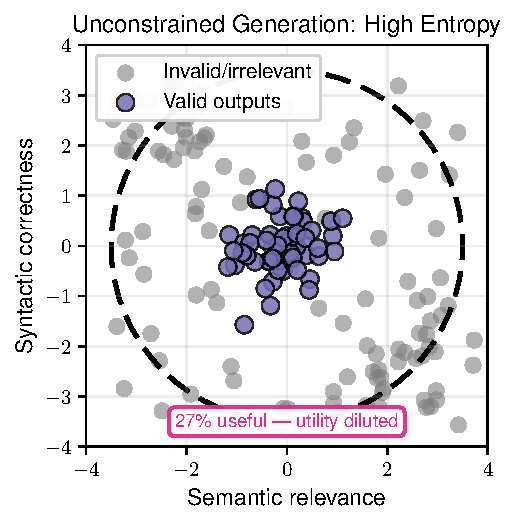
\includegraphics[width=0.8\linewidth]{code/figures/ch11_optimization_geometry/fig_11_2a_unconstrained.pdf}
\caption{Unconstrained generation has high entropy: many outputs are off-format or irrelevant, diluting utility.}
\label{fig:gen_unconstrained}
\end{figure}

\begin{figure}[t]
\centering
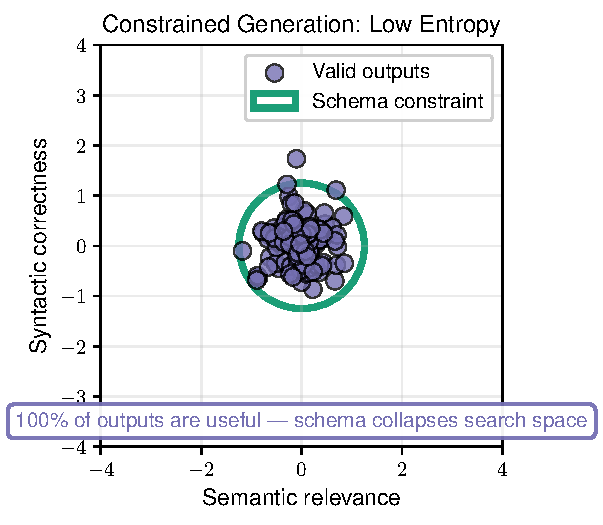
\includegraphics[width=0.8\linewidth]{code/figures/ch11_optimization_geometry/fig_11_2b_constrained.pdf}
\caption{Schema-constrained generation collapses the search space to valid outputs, reducing errors and stabilizing downstream parsing.}
\label{fig:gen_constrained}
\end{figure}

The most direct way to constrain generation is to specify a schema or grammar that defines valid outputs. For structured data like JSON or XML, you provide a schema that specifies required fields, types, and constraints. For code generation, you might specify a grammar that defines valid syntax. For natural language, you might specify a template with placeholders to fill in.

Let's focus on the JSON case because it is common in production systems. Suppose you want the model to output information about a person: name, age, and city. The schema might be:

\begin{verbatim}
{
  "name": string,
  "age": integer,
  "city": string
}
\end{verbatim}

Without constraints, the model might output valid JSON that does not match this schema (missing fields, wrong types, extra fields) or invalid JSON altogether (unmatched braces, unquoted keys). With constraints, you guide the generation process to only produce outputs that conform to the schema.

There are two main approaches to enforcing schemas. The first is post-hoc validation: let the model generate freely, then check if the output matches the schema. If it does not, retry with a modified prompt or use a fallback. This is simple but wasteful because you spend tokens on invalid outputs and then discard them.

The second approach is constrained decoding: modify the generation process itself to only sample tokens that maintain schema validity. At each step, you check which tokens would keep the partially generated output on a path toward a valid completion, and you mask out (set probability to zero) any tokens that would violate the schema. This guarantees that the final output is valid by construction.

Constrained decoding is elegant but has implementation complexity. You need to track the current state of the partially generated output and compute which tokens are valid at each step. For simple schemas, this can be done with a finite automaton. For complex schemas with nested structures and conditional fields, you may need a full parser that runs alongside generation.

A middle-ground approach is to use few-shot prompting with schema examples and then apply lightweight post-hoc validation. You show the model several examples of valid outputs, which biases it toward producing similar outputs. Then you check the output against the schema and retry if necessary. This works well in practice because modern models are good at following patterns, so most outputs will be valid after seeing a few examples.

\vspace{1.5em}

\begin{examplebox}
\textbf{Constrained JSON Generation}

\vspace{0.5em}

Suppose you are building a system that extracts structured information from customer reviews. Given a review, you want to output JSON with fields for sentiment (positive/negative/neutral), rating (1-5), and key phrases (list of strings).

\vspace{0.5em}

\textbf{Unconstrained approach:}

Prompt: "Extract sentiment, rating, and key phrases from this review: [review text]. Output as JSON."

The model might produce:

\begin{verbatim}
{
  "sentiment": "good",
  "rating": "4 stars",
  "phrases": "great product, fast shipping"
}
\end{verbatim}

This looks reasonable but has problems: "good" is not in the expected set \{positive, negative, neutral\}, "4 stars" is a string instead of an integer, and "phrases" is a single string instead of a list.

\vspace{0.5em}

\textbf{Constrained approach with few-shot prompting:}

Prompt: "Extract sentiment, rating, and key phrases from reviews. Use this format:

Example 1:
Review: 'Love this product! Arrived quickly.'
Output: \{\"sentiment\": \"positive\", \"rating\": 5, \"phrases\": [\"love this product\", \"arrived quickly\"]\}

Example 2:
Review: 'Disappointed. Quality is poor.'
Output: \{\"sentiment\": \"negative\", \"rating\": 2, \"phrases\": [\"disappointed\", \"quality is poor\"]\}

Now extract from: [review text]"

The model now produces:

\begin{verbatim}
{
  "sentiment": "positive",
  "rating": 4,
  "phrases": ["great product", "fast shipping"]
}
\end{verbatim}

This matches the schema. The few-shot examples constrained the output space implicitly, and you can add post-hoc validation to catch any remaining errors.
\end{examplebox}

\vspace{1.5em}

\subsection{Lightweight Validation: Type Checks and Range Checks}

Even with constrained generation or schema-guided prompting, you should validate outputs before using them downstream. Validation is your last line of defense against format drift and hallucination.

Lightweight validation means checking basic properties that can be verified quickly without deep semantic understanding. Type checks ensure that fields have the expected types: strings are strings, numbers are numbers, lists are lists. Range checks ensure that numeric values fall within sensible bounds: ages are between 0 and 150, probabilities are between 0 and 1, ratings are between 1 and 5.

Format checks ensure that strings match expected patterns: email addresses contain '@', URLs start with 'http://' or 'https://', dates are in ISO format. These checks are fast (regular expressions, simple comparisons) and catch most common errors.

Beyond these basic checks, you can add domain-specific validation. If you are extracting medical codes, check that they exist in the official codebook. If you are generating SQL queries, check that table and column names are valid. If you are producing citations, check that the cited works exist in your database.

The principle is to fail fast and fail gracefully. When validation detects an error, do not silently ignore it or pass the malformed output downstream. Instead, either retry generation with a modified prompt (adding instructions to fix the specific error), or fall back to a simpler approach (returning a structured error instead of corrupt data).

\vspace{1em}

\subsection{Unit-Test Snippets for Code Generation}

Code generation deserves special attention because code has precise semantics and incorrect code can have serious consequences. Validation for code goes beyond syntax checking to include functional correctness.

One effective pattern is to generate unit tests alongside the code and run them immediately. If you ask the model to implement a function, also ask it to generate test cases that the function should pass. Then execute the tests in a sandboxed environment. If the tests pass, you have some confidence that the code is correct. If they fail, you can provide the test results back to the model and ask it to fix the code.

This pattern leverages the model's ability to understand specifications and expected behavior. By generating tests, the model makes its understanding explicit, and execution provides a ground truth signal about correctness. This is more reliable than static analysis alone because it catches semantic errors that type systems miss.

A key practical detail is sandboxing. You must execute generated code in an isolated environment where it cannot access sensitive resources, modify state, or run indefinitely. Standard practices include running in containers with limited permissions, imposing CPU and memory limits, and using timeouts to kill runaway executions.

Another detail is determinism. Tests that depend on randomness, current time, or external state can produce flaky results. Encourage the model to generate deterministic tests by providing seed values for random number generators and using fixed timestamps in examples.

\vspace{2em}

%==========================
\section{Keep the Loop Stable}
%==========================

Systems that rely on model outputs often form feedback loops. The model's outputs influence future inputs, either directly (the model's previous outputs are included in the next prompt) or indirectly (the model's outputs are used to update a database or UI that the model later queries). These loops can be stable or unstable, and instability manifests as drift: the model's behavior gradually shifts over time in ways you did not anticipate.

\vspace{1em}

\subsection{Monitoring for Drift: Three Signals to Watch}

Drift is the enemy of reliable systems, and it comes in three main flavors. Input distribution drift occurs when the distribution of queries or prompts changes over time. Loss drift occurs when the model's performance on your task degrades. Calibration drift occurs when the model's confidence scores become less reliable.

Let's examine each in turn, starting with input distribution drift. This is about detecting when the types of queries you receive shift away from what you expected. For example, if you built a customer support chatbot trained on queries from January, and in June you start receiving queries about a new product feature, your input distribution has shifted.

You can detect input drift by monitoring summary statistics of your input embeddings. Compute embeddings of incoming queries using the same encoder you use for retrieval. Track the mean and covariance of these embeddings over time. If the mean drifts significantly or the covariance structure changes, you have distribution shift. You can quantify this drift using metrics like Maximum Mean Discrepancy (MMD) or KL divergence between the current distribution and a reference distribution.

A simpler approach is to track the frequency of out-of-vocabulary terms or rare n-grams. If you start seeing many queries with terms that were rare in training, this signals that the input distribution is shifting. You can set thresholds on these frequencies and trigger alerts when they are exceeded.

Loss drift is about tracking whether the model's outputs are getting worse over time. This is harder to measure in production because you often do not have ground truth labels for real queries. But you can use proxy signals: track the rate of retries (queries that users rephrase after getting a bad answer), track explicit feedback (thumbs up/down), or maintain a small labeled evaluation set that you re-evaluate periodically.

For generative tasks, you can also track output quality metrics like perplexity, length, or diversity. If average perplexity increases, the model is becoming less confident. If average length increases, the model might be generating more verbose or repetitive outputs. If diversity decreases (measured by the number of unique n-grams), the model might be collapsing to generic responses.

Calibration drift is subtle but important. It occurs when the relationship between the model's confidence scores and its actual accuracy changes. A well-calibrated model should be correct 70\% of the time on inputs where it reports 70\% confidence. Calibration drift means this relationship breaks down: the model reports high confidence but is often wrong, or vice versa.

You can monitor calibration by binning predictions by confidence and tracking accuracy within each bin. If accuracy within a bin deviates significantly from the bin's confidence level, calibration has drifted. We will explore calibration in depth in Chapter 13, but for monitoring purposes, you can use simple binned calibration error as a signal.

\vspace{1.5em}

\begin{figure}[t]
\centering
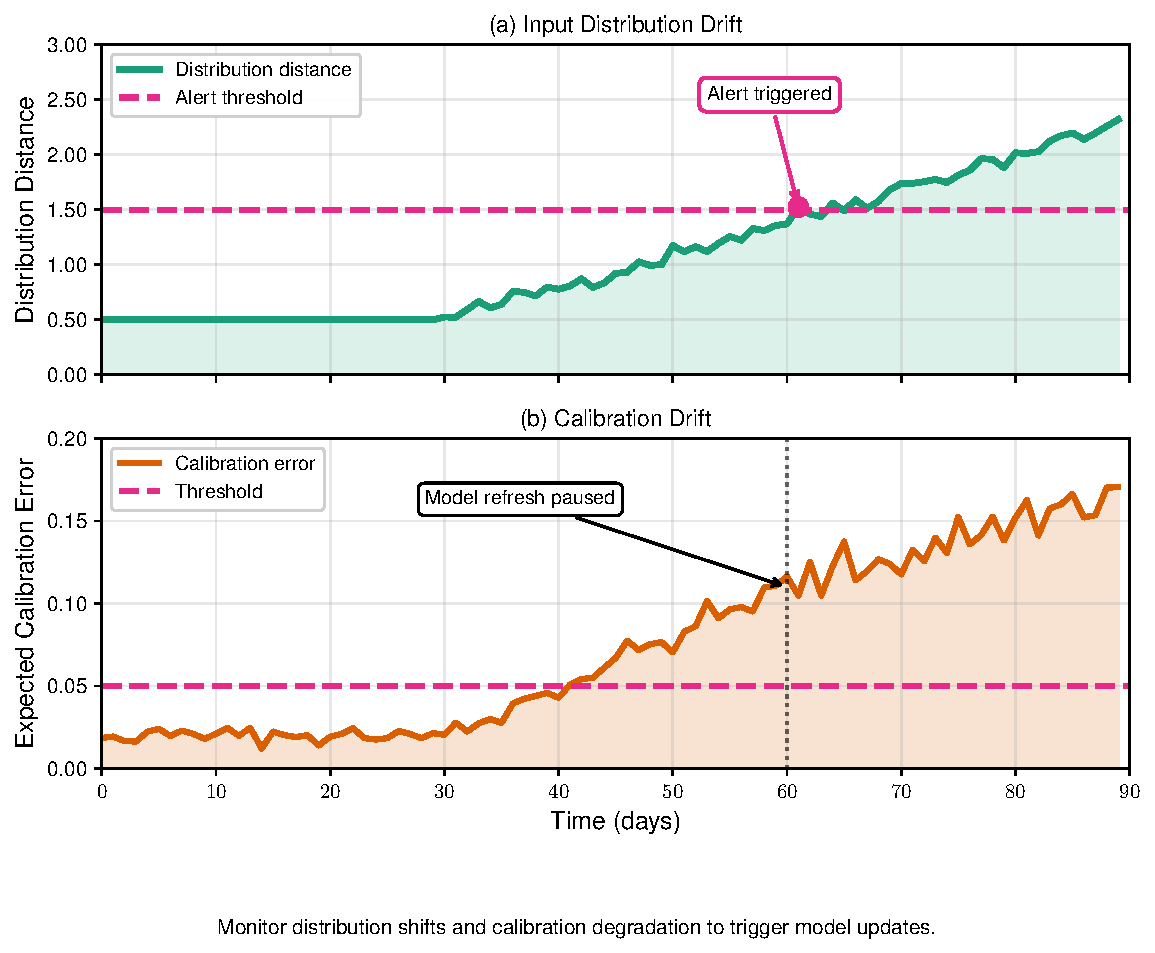
\includegraphics[width=\linewidth]{code/figures/ch11_optimization_geometry/fig_11_3_drift_monitoring.pdf}
\caption{Monitor for drift using multiple signals: input distribution shift, degradation in performance proxies, and calibration error. Each highlights a different failure mode.}
\label{fig:drift_monitoring}
\end{figure}

\begin{geometrylens}
\textbf{Drift as Geometric Motion in Representation Space}

\vspace{0.5em}

Input distribution drift can be visualized as movement in the space of embeddings. Training data defines a region in embedding space where the model is reliable. As inputs drift, they move toward the boundary or outside of this region, where the model's behavior is less predictable.

\vspace{0.5em}

You can formalize this geometrically using the Mahalanobis distance: compute the covariance matrix of training embeddings, and measure how far test embeddings are from the training distribution center in units of standard deviation. Inputs with large Mahalanobis distance are out-of-distribution and more likely to produce unreliable outputs.

\vspace{0.5em}

Calibration drift has a geometric interpretation too. Well-calibrated models have level sets of confidence that align with level sets of accuracy. When calibration drifts, these level sets diverge: regions of high confidence no longer correspond to regions of high accuracy. Monitoring calibration is about detecting when this geometric alignment breaks down.
\end{geometrylens}

\vspace{1.5em}



\subsection{Designing Graceful Fallbacks}

When you detect drift or uncertainty, the system should not fail catastrophically. Instead, it should degrade gracefully by falling back to simpler, more reliable behaviors. This is the engineering analog of selective prediction from Chapter 9: when you cannot make a confident prediction, abstain or fall back.

There are several fallback strategies, arranged from most to least informative. Re-asking is the first fallback: when the model produces a low-confidence output, retry the query with a modified prompt. You might add constraints ("answer in one sentence"), provide examples ("here are two similar cases and their answers"), or simplify the query ("first tell me X, then we'll discuss Y").

Re-asking exploits the fact that generation is stochastic: different samples from the model's distribution may have different quality. By sampling multiple times and using validation or confidence scores to select the best output, you can improve reliability without changing the model.

The second fallback is to simplify the task. If the model struggles with a complex query, break it into simpler sub-queries. Instead of asking "analyze this document and summarize the key risks, opportunities, and recommendations," ask three separate questions: "what are the key risks?", "what are the opportunities?", "what are your recommendations?" Then combine the answers. This reduces the complexity of each individual generation and often improves quality.

The third fallback is to retrieve more context. If the model gives a low-confidence answer, it might be because it lacks information. Retrieve additional documents, provide more examples, or query a knowledge base. This is the Bayesian move: acquire more evidence to reduce posterior uncertainty.

The fourth fallback is to abstain and escalate to a human. If confidence remains low even after retries, simplification, and retrieval, the honest response is "I don't know." Return a structured message indicating that the query could not be answered reliably, along with any partial information that might be useful. In production systems with human oversight, this query can be routed to a person for review.

Each fallback has a cost: re-asking costs latency and tokens, simplification costs interaction overhead, retrieval costs both latency and infrastructure, and escalation costs human time. The key is to order fallbacks by their cost-to-benefit ratio and trigger them based on confidence thresholds.

\vspace{1.5em}

\begin{figure}[t]
\centering
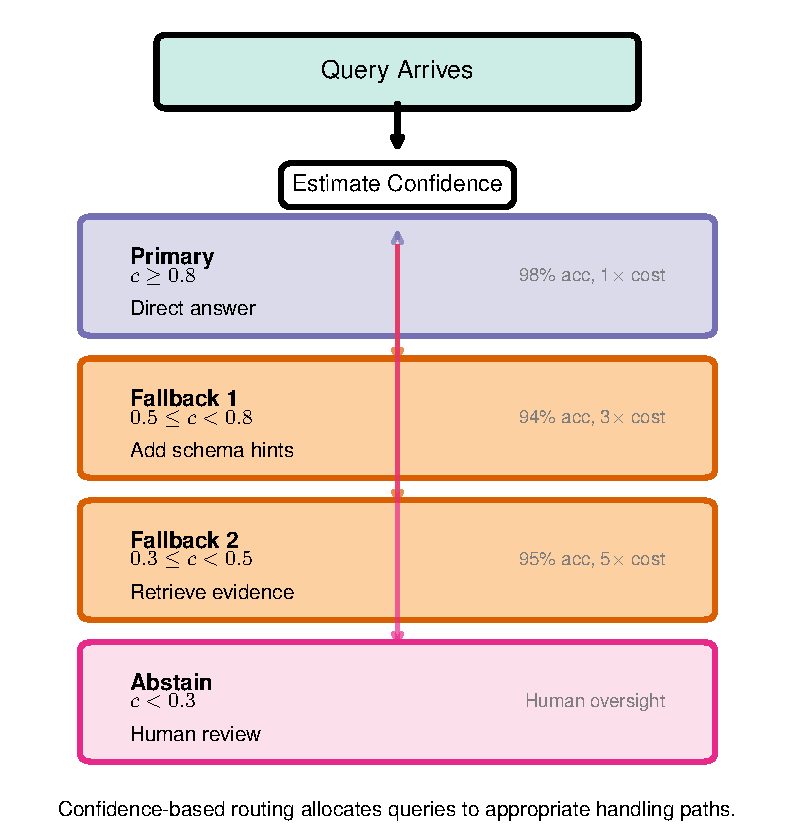
\includegraphics[width=0.9\linewidth]{code/figures/ch11_optimization_geometry/fig_11_4_routing_flow.pdf}
\caption{Confidence-based routing and fallbacks: answer directly when confidence is high, add schema hints on moderate confidence, retrieve evidence when low, and abstain to human review at very low confidence.}
\label{fig:routing_flow}
\end{figure}

\begin{examplebox}
\textbf{Fallback Cascade for Question Answering}

\vspace{0.5em}

Suppose you have a question-answering system with a target of 95\% accuracy. You observe that when the model's maximum token probability is above 0.8, accuracy is 98\%. When it is between 0.5 and 0.8, accuracy is 90\%. When it is below 0.5, accuracy drops to 70\%.

\vspace{0.5em}

Design a fallback cascade:

\vspace{0.5em}

\textbf{Primary path (confidence $\geq$ 0.8):} Return the answer directly. Expected accuracy: 98\%.

\vspace{0.5em}

\textbf{First fallback (confidence 0.5-0.8):} Re-ask with a constraint: "Answer in one sentence using only information you are certain about." Sample three times and select the answer with highest confidence. This improves accuracy from 90\% to approximately 93\% (empirically measured on your evaluation set).

\vspace{0.5em}

\textbf{Second fallback (confidence 0.3-0.5):} Retrieve additional context from your knowledge base and re-ask. This improves accuracy to approximately 94\%.

\vspace{0.5em}

\textbf{Third fallback (confidence $<$ 0.3):} Abstain. Return \{\"answer\": null, \"reason\": \"insufficient confidence\", \"suggested\_action\": \"rephrase query or provide more context\"\}.

\vspace{0.5em}

By routing queries through this cascade based on confidence, you achieve overall accuracy above 95\% while minimizing the cost of expensive fallbacks. Most queries (60\%) take the primary path. Some (30\%) need the first fallback. Few (8\%) need the second fallback. Very few (2\%) result in abstention.
\end{examplebox}

\vspace{1.5em}

\subsection{Feedback Loops and Self-Amplification}

Some systems create feedback loops where the model's outputs influence its future inputs. This happens in conversational systems (where the model's responses become part of the conversation history), in retrieval-augmented generation (where the model's outputs might be added to the retrieval corpus), and in iterative refinement (where the model critiques and improves its own outputs).

Feedback loops can amplify errors. If the model generates a slightly incorrect fact and that fact is added to the retrieval corpus, future queries might retrieve that incorrect fact, leading the model to generate it again with higher confidence. Over time, errors can become entrenched.

The information-theoretic view is that feedback loops can concentrate probability mass on wrong answers. Initially, the model's distribution over answers might be broad, with the correct answer having slightly higher probability than incorrect alternatives. But if the model samples an incorrect answer and that answer is fed back as context, the distribution shifts: the incorrect answer now has higher probability because it appears in the context. Repeated feedback amplifies this shift until the incorrect answer dominates.

\begin{figure}[t]
\centering
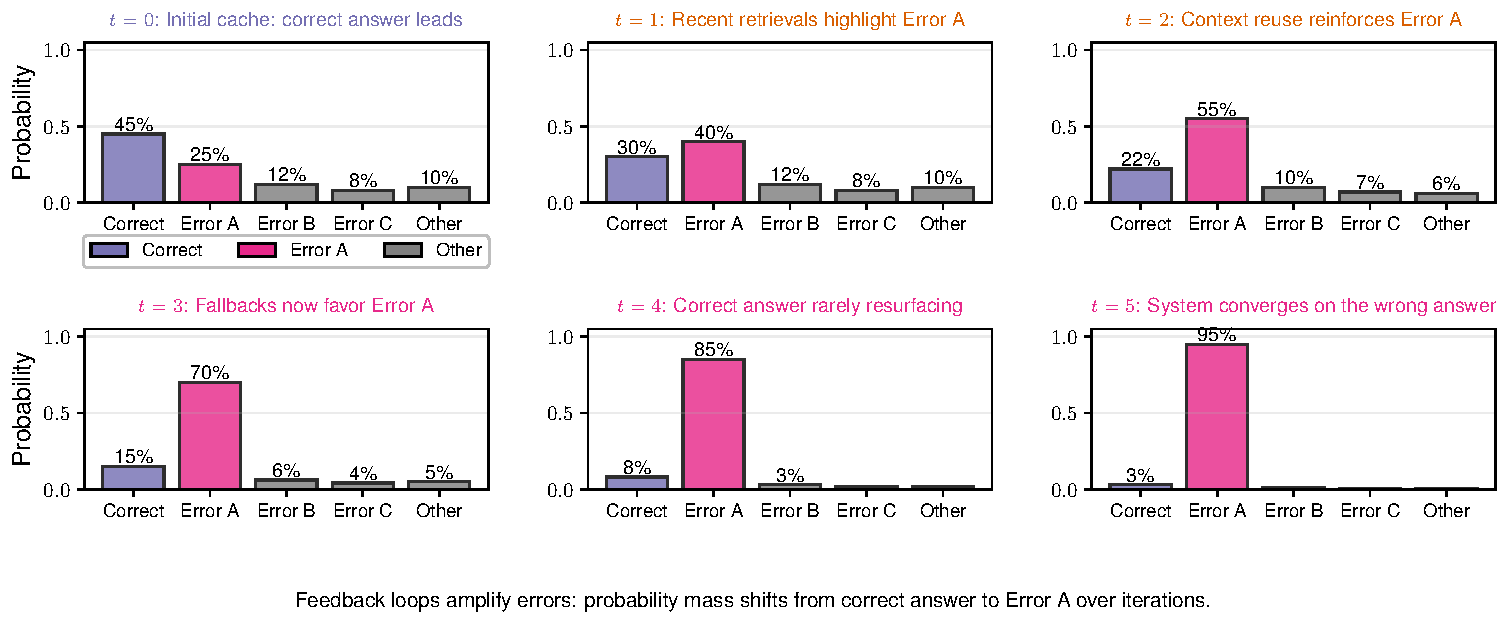
\includegraphics[width=\linewidth]{code/figures/ch11_optimization_geometry/fig_11_7_feedback_amplification.pdf}
\caption{Unfiltered feedback loops amplify errors: repeated reuse of mistaken outputs shifts probability mass toward the wrong answer unless you validate, diversify, or reset.}
\label{fig:feedback_amplification}
\end{figure}

To keep feedback loops stable, you need to prevent error amplification. One approach is to filter what gets fed back. Only include high-confidence outputs in the feedback loop, and validate them before inclusion. If you are adding model outputs to a retrieval corpus, require that they match a schema, pass validation checks, and have confidence above a high threshold.

Another approach is to add diversity. Instead of always feeding back the model's top-scoring output, sample from its distribution and include multiple alternatives. This prevents premature convergence and maintains the breadth of the posterior.

A third approach is periodic resets. Clear the feedback loop periodically and restart from a clean slate. For conversational systems, this means starting new conversations rather than maintaining indefinitely long context. For retrieval corpora, this means periodically removing model-generated content and rebuilding from ground truth sources.

\vspace{2em}

%==========================
\section{Design for Efficiency}
%==========================

Information is not free. Every token you process costs compute, every retrieval costs latency, and every model call costs money. Designing efficient systems means allocating these limited resources where they provide the most value. This is the information budgeting framework from Chapter 1 applied to system design.

\vspace{1em}

\subsection{Budgeting Tokens and Latency}

The most direct resource constraint is tokens. Whether you are using a local model with limited context or a cloud API with per-token pricing, you have a budget for how many tokens you can afford per query. The question is: how do you allocate this budget?

The principle is to spend tokens where they reduce entropy the most. If your goal is to produce a high-quality answer, spend tokens on providing relevant context and detailed instructions. If your goal is to classify intent, you might need fewer tokens because the output space is small. If your goal is to generate creative content, you might need more tokens because the output space is large.

Token budgeting has two main components: input tokens and output tokens. Input tokens include the prompt, retrieved context, and any few-shot examples. Output tokens are the generated response. You control input tokens by choosing how much context to include and how many examples to provide. You control output tokens by setting maximum generation length and stopping criteria.

A practical approach is to set a total token budget per query and allocate it between input and output based on the task. For retrieval-heavy tasks (question answering with documents), spend 80\% of the budget on input and 20\% on output. For generation-heavy tasks (creative writing, summarization), spend 50-50 or even 40-60 in favor of output.

\begin{figure}[t]
\centering
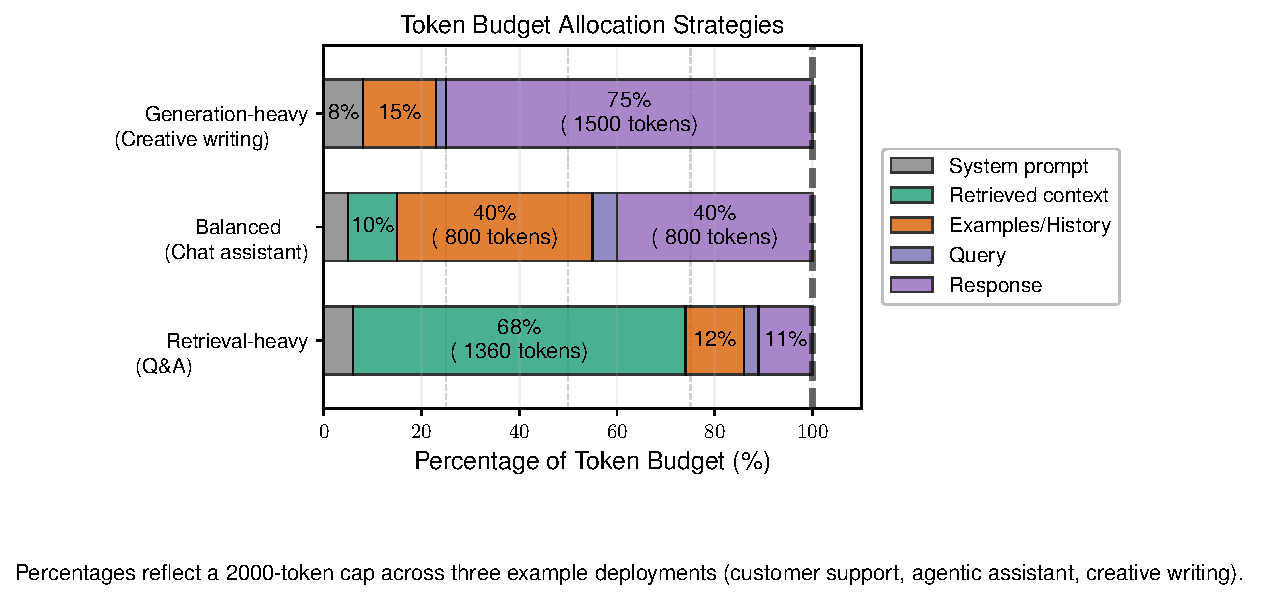
\includegraphics[width=\linewidth]{code/figures/ch11_optimization_geometry/fig_11_5_token_budget.pdf}
\caption{Token budget strategies: allocate tokens where they reduce uncertainty most (context for retrieval-heavy tasks, response length for generation-heavy tasks).}
\label{fig:token_budget}
\end{figure}

Within the input budget, prioritize high-relevance content. If you retrieve ten documents but can only afford to include five in the context, rank them by relevance and include the top five. If you have a long conversation history but can only include the last ten turns, use a sliding window or extract a summary of earlier turns.

Latency is the other critical resource. Users tolerate a few seconds of latency for complex queries, but not tens of seconds. Latency has two main sources: model inference time and retrieval time. You can reduce inference time by using faster models (smaller or more efficient architectures), batching multiple queries together, or caching common prompts. You can reduce retrieval time by using faster vector stores, indexing carefully, and caching frequent queries.

There is a tradeoff between latency and quality. Faster models are often less accurate. Less retrieval means less context. Shorter generation means less detailed answers. The key is to understand this tradeoff for your specific task and tune for the latency-quality point that meets your requirements.

\vspace{1em}

\subsection{Batching, Streaming, and Caching Common Work}

Batching is about amortizing fixed costs over multiple queries. If you have overhead per model call (loading weights, initializing state), processing queries one at a time wastes resources. Instead, collect a batch of queries and process them together. This is especially effective for retrieval: if ten users ask similar questions around the same time, you can retrieve once and share the results.

The challenge with batching is latency. Waiting to accumulate a full batch adds delay. The optimal batch size depends on your latency budget and the rate of incoming queries. For high-throughput systems, large batches (32, 64, or more) make sense. For interactive systems, small batches (1-4) or no batching may be necessary.

Streaming is an alternative to waiting for complete generation. Instead of generating the full response and then returning it, stream tokens as they are generated. The user sees partial results immediately, which improves perceived latency even if total latency is unchanged. Streaming also lets you implement early stopping: if the user indicates the answer is sufficient, you can halt generation and save tokens.

Streaming has complexity costs. You need to handle partial outputs gracefully, buffer appropriately, and deal with network interruptions. But for long-form generation, the perceived latency improvement is often worth it.

Caching common work is the most effective efficiency technique. Identify computations that are repeated across queries and cache their results. For example, if many queries involve the same few-shot examples, encode those examples once and cache the embeddings. If many queries retrieve from the same documents, precompute document embeddings and store them in an index. If many queries use the same system prompt, cache the key-value attention states for that prompt so they do not need to be recomputed.

Modern transformer implementations support this through key-value caching: once you have processed a prompt, you cache the attention keys and values, and future queries that share a prefix can reuse them. This is particularly effective for multi-turn conversations where each turn shares the history with previous turns.

\vspace{1.5em}

\begin{keyinsight}
Caching is about exploiting redundancy in your query distribution. High redundancy (many similar queries) makes caching highly effective. Low redundancy (every query is unique) makes caching useless. The optimal caching strategy depends on the entropy of your query distribution: low entropy means more caching, high entropy means less.
\end{keyinsight}

\vspace{1.5em}

\subsection{The "Small, Fast, Certain" Path vs "Big, Slow, Maybe" Path}

Different queries need different amounts of resources. Some are simple and can be answered quickly with high confidence. Others are complex and require extensive computation. A robust system should route queries to the appropriate path.

The "small, fast, certain" path is for queries where the answer is well-known and confidence is high. Use a smaller model, skip retrieval, generate a short response. The goal is to minimize latency and cost while maintaining reliability.

The "big, slow, maybe" path is for queries where the answer is uncertain or complex. Use a larger model, retrieve extensively, generate a longer response, apply multiple fallbacks. The goal is to maximize quality even at the cost of latency and compute.

The routing decision can be made using heuristics or learned. Heuristic routing uses simple rules: if the query is short and contains no named entities, take the fast path. If the query is long or contains "explain" or "analyze," take the slow path. Learned routing trains a small classifier on query features to predict which path will succeed.

This two-path design is a specific instance of a general principle: allocate resources adaptively based on task difficulty. Easy tasks get fewer resources, hard tasks get more. This is more efficient than treating all tasks the same because you avoid wasting resources on easy tasks and avoid under-resourcing hard tasks.

\begin{figure}[t]
\centering
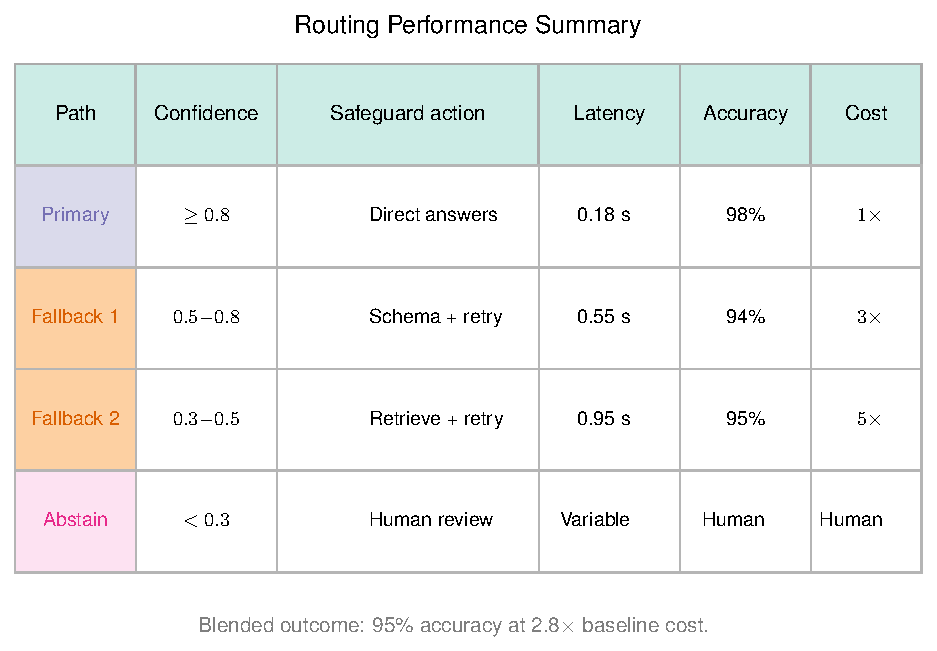
\includegraphics[width=\linewidth]{code/figures/ch11_optimization_geometry/fig_11_6_routing_metrics.pdf}
\caption{Routing performance summary: confidence thresholds map to safeguards, latency, accuracy, and cost, enabling an adaptive blend that meets quality targets.}
\label{fig:routing_metrics}
\end{figure}

The information-theoretic perspective is that different queries have different posterior entropy. Queries with low posterior entropy (the model is confident) need fewer resources to answer well. Queries with high posterior entropy (the model is uncertain) need more resources to reduce entropy sufficiently. By estimating posterior entropy from query features or model outputs, you can route adaptively.

\vspace{2em}

%==========================
\section{The Minimal Architecture: One Page of Enduring Patterns}
%==========================

Let's synthesize what we have learned into a minimal architecture that captures the patterns that endure. This is not a specific framework or codebase. It is a conceptual model that you can draw on one page and adapt to your domain.

\vspace{1em}

\subsection{The Four-Stage Pattern: Encode, Budget, Verify, Act}

Here is the pattern. Every robust system for language or generative AI follows these four stages, though the implementation details differ.

\textbf{Stage 1: Encode.} Take the input (query, document, image) and encode it into a representation that captures relevant information. For text, this might be embeddings from a language model. For structured data, this might be feature vectors. The encoding stage compresses the input into a form that downstream components can work with efficiently.

From an information perspective, encoding is lossy compression. You are discarding irrelevant details and retaining what matters for the task. The quality of this compression determines how much information is available to later stages. Good encoders preserve task-relevant information and discard noise.

\textbf{Stage 2: Budget.} Decide how many resources to allocate to this query. Should you retrieve? If so, how much? Which model should you use? How many tokens can you afford? The budgeting stage makes these allocation decisions based on the encoded representation and any metadata (user priority, historical performance, confidence estimates).

From an information perspective, budgeting is about allocating capacity to reduce entropy where it matters most. You have limited capacity (context length, compute, latency), and you need to allocate it to maximize the reduction in uncertainty about the correct answer.

\textbf{Stage 3: Verify.} After generation, check that the output is well-formed and plausible. This includes schema validation, type checks, range checks, and any domain-specific validation. If verification fails, trigger fallbacks (re-ask, retrieve, simplify, or abstain).

From an information perspective, verification is about ensuring that the sampled output actually comes from the high-probability region of the distribution. Models can occasionally sample from low-probability tails, producing nonsense. Verification catches these samples and triggers correction.

\textbf{Stage 4: Act.} Use the verified output to take action. This might mean returning a response to the user, updating a database, calling an API, or triggering another system. The action stage is where outputs have consequences, so it is critical that inputs to this stage have been verified.

From an information perspective, acting is about converting information (the model's output) into effects in the world. The quality of these effects depends on the accuracy of the information, which is why verification must precede action.

\vspace{1.5em}

\begin{figure}[t]
\centering
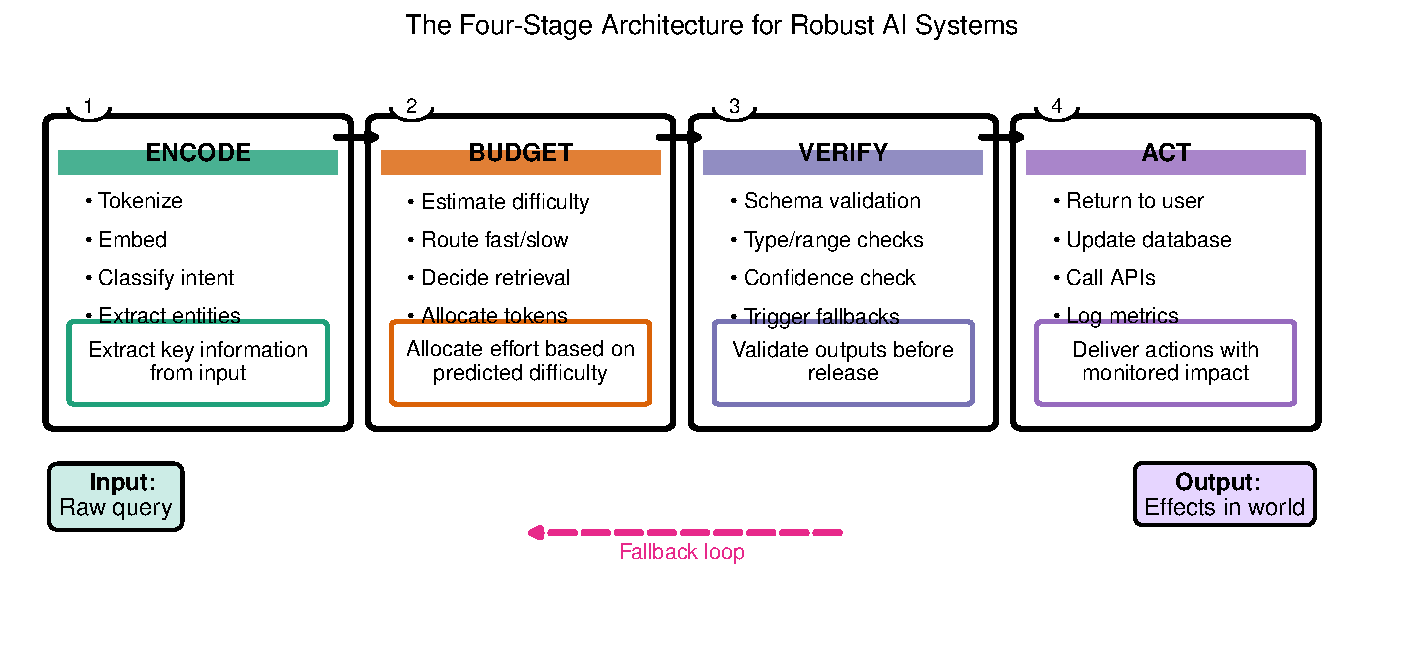
\includegraphics[width=\linewidth]{code/figures/ch11_optimization_geometry/fig_11_8_four_stage_architecture.pdf}
\caption{The four-stage architecture that endures: encode inputs, budget resources, verify outputs, then act—most real systems elaborate this loop.}
\label{fig:four_stage_architecture}
\end{figure}

\begin{examplebox}
\textbf{The Four Stages in a Customer Support System}

\vspace{0.5em}

Let's trace a query through the four stages.

\vspace{0.5em}

\textbf{Input:} "My order hasn't arrived and it's been a week. Can you help?"

\vspace{0.5em}

\textbf{Encode:} Embed the query. Classify intent as "order status inquiry" with high confidence. Extract entity "one week" as time reference. Determine that retrieval is needed (specific order status).

\vspace{0.5em}

\textbf{Budget:} Allocate high priority because sentiment analysis suggests frustration. Retrieve order history for the user. Use a medium-sized model (fast enough for real-time, accurate enough for customer-facing response). Allow up to 150 tokens for the response.

\vspace{0.5em}

\textbf{Verify:} Generate response: \{\"status\": \"shipped\", \"expected\_delivery\": \"2024-01-15\", \"tracking\": \"XYZ123\", \"message\": \"Your order shipped on Jan 12 and should arrive by Jan 15. You can track it here: [link]\"\}. Check schema: all required fields present, types correct. Check tracking number exists in database: pass. Check expected delivery date is in the future: pass.

\vspace{0.5em}

\textbf{Act:} Return response to user. Log interaction for monitoring. If expected delivery date is more than 3 days away, trigger proactive outreach from customer service team.

\vspace{0.5em}

If verification had failed (e.g., tracking number not found in database), fallback: retrieve again with broader search, or escalate to human agent if still no match.
\end{examplebox}

\vspace{1.5em}

\subsection{Why This Pattern Endures}

This four-stage pattern endures because it is grounded in fundamental constraints that do not change with model architectures or scaling laws. Encoding will always be necessary because raw inputs are too high-dimensional to process directly. Budgeting will always be necessary because resources are finite. Verification will always be necessary because models are stochastic and can fail. Action will always be necessary because systems must interact with the world.

Different systems implement these stages differently. A real-time translation system might use lightweight encoding (simple tokenization), minimal budgeting (fixed resources per query), fast verification (basic grammar checks), and direct action (display translation). A medical diagnosis system might use rich encoding (multimodal fusion of images and text), careful budgeting (allocate more resources to uncertain cases), extensive verification (check against medical databases), and cautious action (recommend specialist consultation rather than direct diagnosis).

But the pattern is the same. By organizing your system around these four stages, you create clear boundaries between concerns. Encoding is about representation. Budgeting is about resource allocation. Verification is about correctness. Action is about effects. Each stage has a well-defined input and output, making the system easier to understand, test, and maintain.

\vspace{1em}

\subsection{What Endures: Compression and Constraint}

Let me distill the lesson of this chapter to its essence. Robust systems are organized conversations between compression and constraint.

Compression is about reducing entropy, finding structure, and representing information efficiently. This is what models do when they learn. This is what retrieval does when it selects relevant context. This is what encoding does when it maps inputs to representations.

Constraint is about restricting possibilities, ruling out invalid states, and ensuring correctness. This is what schemas do when they specify valid outputs. This is what verification does when it checks properties. This is what budgeting does when it limits resource use.

The conversation between compression and constraint goes like this. Compression says: here are many possibilities, let me find the most likely one. Constraint says: among these possibilities, only some are acceptable, let me rule out the rest. Together, they guide the system toward outputs that are both probable (compression) and valid (constraint).

This is not specific to language models or transformers or any particular architecture. It is a general principle for building systems that operate in uncertain environments with limited resources. As models evolve and scale, the specifics of compression (what architecture, what training method) and constraint (what validation, what schemas) will change. But the pattern of organizing systems around their conversation will endure.

\vspace{2em}

%==========================

\begin{pausebox}
\textbf{Pause: Consolidating System Design Principles}

\vspace{0.5em}

Before moving forward, reflect on the patterns we have explored:

\vspace{0.5em}

Can you explain why retrieval should be triggered by posterior entropy rather than always or never? Can you describe the tradeoff between constrained decoding and post-hoc validation? Do you understand why feedback loops can amplify errors and how to prevent this? Can you articulate the principle behind the "small, fast, certain" versus "big, slow, maybe" routing decision?

\vspace{0.5em}

Most importantly, can you see how all these patterns are grounded in information theory? Retrieval is evidence acquisition. Constraints reduce output entropy. Monitoring detects distribution shift. Efficiency is resource allocation under capacity constraints. These are not engineering heuristics—they are applications of fundamental principles.

\vspace{0.5em}

If these connections feel clear, you are ready for the final chapters on calibration, scaling, and deployment. If anything still feels uncertain, revisit the relevant section. The patterns in this chapter will appear again when we discuss calibration (Chapter 13), scaling decisions (Chapter 10), and production systems (Chapter 14).
\end{pausebox}

\vspace{1em}

This chapter has translated information-theoretic principles into practical system design patterns. We explored how to acquire information through retrieval (evidence acquisition to reduce posterior entropy), how to constrain outputs (restricting generation to valid subspaces), how to maintain stability (monitoring for drift and designing fallbacks), how to allocate resources efficiently (budgeting tokens and latency where they matter), and how to organize these patterns into a minimal architecture that endures across model families and problem domains.

The key insight is that robust systems are organized conversations between compression and constraint. Models compress by learning structure and predicting probable outputs. Systems constrain by validating outputs and enforcing invariants. The interplay between these forces determines reliability. Too much compression without constraint leads to hallucination and format drift. Too much constraint without compression leads to brittle, unscalable systems. The right balance is dynamic, adapting to query difficulty, resource availability, and confidence levels.

In the next chapter, we will explore scaling laws: how performance improves with more compute, data, and parameters. The information budgeting framework from this chapter will help us understand why scaling laws exist and how to navigate the tradeoffs between different resources. We will see that scaling is ultimately about allocating information capacity efficiently, and the patterns we have learned here—adaptive routing, budgeting, and monitoring—apply at the level of training as well as inference.

\vspace{1em}

\begin{pausebox}
\textbf{Key Takeaways from Chapter 11}

Retrieval is evidence acquisition: retrieve when posterior entropy is high relative to retrieval cost. Constrain generation through schemas, validation, and examples to prevent format drift and ensure correctness. Monitor for drift in inputs, loss, and calibration; design fallback cascades that degrade gracefully. Budget tokens and latency adaptively based on query difficulty and confidence. Organize systems around four stages: encode (compress inputs), budget (allocate resources), verify (ensure correctness), act (produce effects). Robust systems are conversations between compression (finding probable outputs) and constraint (ensuring valid outputs). These patterns endure because they are grounded in information theory, not tied to specific architectures or trends.
\end{pausebox}
